%%%%%%%%%%%%%%%%%%%%%%%%%%%%%%%%%%%%%%%%%%%%%%%%%%%%%%%%%%%%%%%%%%%%%%%%%%%%%%%
%% Supporting Information
%% TODO:
%%    TODO: Free energy corrections to OER intermediates, OER mechanism
%%    TODO: Is there any cross-validation happening here? I don't think so
%%%%%%%%%%%%%%%%%%%%%%%%%%%%%%%%%%%%%%%%%%%%%%%%%%%%%%%%%%%%%%%%%%%%%%%%%%%%%%%


% #############################################################################
\section{Active Learning ML Section}  % #######################################
% #############################################################################
%
% #############################################################################
% | - Active Learning ML Section

\subsection{Candidate space generation}
% | - Candidate space generation
The candidate for IrO2 and IrO3 were generated from existing experimental structures in the OQMD and Materials Project databases.
%
There are TEMP unique AB2 structures (or multiples, e.g. A2B4)
%
Of those we found 697 unique AB2 prototypes (unique SG/Wyckoff combination) in OQMD/MP
%

% #############################################################################
% VOLUME Pre-optimization of static prototypes

% __|

\subsection{Gaussian process regression model}
% | - Gaussian process regression model
Relevant details about the ML Gaussian process here  % @Chris

% TODO Check again how I handled the length vectors
The Gaussian Process model utilized a rational quadratic kernel with variable length scales for each dimensino of the feature space.
% CV error of XYZ eV/atom, initial predictions in figure XYZ.
% - Selected 10 structures with lowest prediction-uncertainty for DFT.
% Structures were volume optimized, then fully relaxed, described in methods XYZ.
% - Model retrained with the 10 DFT computed structures ONLY, 271 features->110 features applicable to \ce{IrO_2}->20 principle components for 99.9 percent variance.
% CV error…
% - Repeat until XYZ, final predictions shown in Fig XYZ
% __|

\subsection{Bulk polymorph DFT optimization}
% | - Bulk polymorph DFT optimization
VASP
PBE exchange correlation functional
spin-polarized calculations
plane-wave cutoff of 600 eV

A variable k-point mesh is used such that a kpoint density of at least 20 kpoints per recipricol space dimension.

All bulk systems were run through the following computational recipe to converge the equilibrium structure.
The recipe has 3 distinct phases, and structures are only advanced to the next phase when the previous phase completes without error.
1. A isif 7 calculation to optimize only the volue (initial volume of cell may be really off)
2. 3 consecutive isif 3 relaxations to fully converge the lattice and atomic positions
3. A final isif 2, calculation to relax the atomic coorindates only to avoid errors associated with changing the cell volume with a fixed plane-wave cutoff basis

The final isif 2 step is run with an electronic energy SCF convergence criteria of 1E-6 eV and the ionic relaxation has a tight force convergence criteria of 1E-3 eV/Angstrom
% __|

\subsection{Structural coordination motiff identification}
% | - Structural coordination motiff identification
Several esoteric structural features were found in the DFT optimized structures and can be catogorized as one of two types, legitimate structural motiffs not characterized by the scheme of Waroquiers et. al. \cite{Waroquiers2017}, and arguably non-physical structural artifacts, including:
% TODO Add more of these
- unassociated oxygen atoms
- molecular oxygens in the unit cell
%
% __|

% __|


% #############################################################################
\section{Electrochemical OER Computational Methods}  % ########################
% #############################################################################
%
% #############################################################################
% | - Electrochemical OER Computational Methods

% %%%%%%%%%%%%%%%%%%%%%%%%%%%%%%%%%%%%%%%%%%%%%%%%%%%%%%%%%%%%%%%%%%%%%%%%%%%%%
\subsection{Density Functional Theory Methods}  % %%%%%%%%%%%%%%%%%%%%%%%%%%%%%
% %%%%%%%%%%%%%%%%%%%%%%%%%%%%%%%%%%%%%%%%%%%%%%%%%%%%%%%%%%%%%%%%%%%%%%%%%%%%%
%
% %%%%%%%%%%%%%%%%%%%%%%%%%%%%%%%%%%%%%%%%%%%%%%%%%%%%%%%%%%%%%%%%%%%%%%%%%%%%%
% | - Density Functional Theory Methods
% Get VASP #REF in the ex. word doc. that @Michal shared with me
All OER calculations were performed using density functional theory (DFT) implemented via the Vienna ab-initio simulation package (VASP) and utilizing the PBE exchange-correlation functional.
Dipole corrections were imposed on all non-symmetric slabs.
A 4x4x3 k-point mesh with gamma-point centered Monkshort-packing was used for all slabs.
The plane-wave energy cutoff was 500 eV.

% #COMBAK Figure out how much spacing was used for all slabs
% FIXME Change the A -> Angstrom symbol

% #COMBAK What kind of optimization routine was used? (Newtonian, BFGS?)
All slab calculations maintained a vacuum spacing of <15 A.
% #COMBAK change A -> Angstrom
All structures were relaxed utilizing a TEMP algorithm with a stop criteria being that all atoms satisfy a maximum force threshold of 0.02 eV/A.
% __|



% %%%%%%%%%%%%%%%%%%%%%%%%%%%%%%%%%%%%%%%%%%%%%%%%%%%%%%%%%%%%%%%%%%%%%%%%%%%%%
\subsection{OER Thermodynamic Methodology}  % %%%%%%%%%%%%%%%%%%%%%%%%%%%%%%%%%
% %%%%%%%%%%%%%%%%%%%%%%%%%%%%%%%%%%%%%%%%%%%%%%%%%%%%%%%%%%%%%%%%%%%%%%%%%%%%%
%
% %%%%%%%%%%%%%%%%%%%%%%%%%%%%%%%%%%%%%%%%%%%%%%%%%%%%%%%%%%%%%%%%%%%%%%%%%%%%%
% | - OER Thermodynamic Methodology
Procedure:
- For the top/most stable bulk structures the following procedure was carried out

* Stable stoichiometric terminations were cut from the bulk Stable termination planes were guesstimated via intuition, and the x-ray diffraction pattern tool from Vesta

* Electrochemical surface coverage was elucidated via a surface Pourbaix analysis Need to know the coverage of surface under operating conditions (>1.23 V RHE)

* Thermodynamic/limiting potential analysis of the OER mechanistic pathway Volcano plot, limiting potentials, etc.
% __|



% %%%%%%%%%%%%%%%%%%%%%%%%%%%%%%%%%%%%%%%%%%%%%%%%%%%%%%%%%%%%%%%%%%%%%%%%%%%%%
\subsection{Surface Energy Pourbaix Methodology}  % %%%%%%%%%%%%%%%%%%%%%%%%%%%
% %%%%%%%%%%%%%%%%%%%%%%%%%%%%%%%%%%%%%%%%%%%%%%%%%%%%%%%%%%%%%%%%%%%%%%%%%%%%%
%
% %%%%%%%%%%%%%%%%%%%%%%%%%%%%%%%%%%%%%%%%%%%%%%%%%%%%%%%%%%%%%%%%%%%%%%%%%%%%%
% | - Surface Energy Pourbaix Methodology
Surface energy Pourbaix plots were constructed by calculating the surface energy of each slab by under standard conditions (V=0 and pH=0) and then utilizing the computational hydrogen electrode to compute the potential dependence of the surfaces.

Surface energy calculations were performed for various facets for slabs of increasing thickness.
The bulk energy was then extracted by fitting the total energy of the slabs against the number of layers as explained in REF2.
This was  done to avoid common issues of surface energy divergence associated with using a separate bulk energy calculation.

The sensitivity of a given slab to an applied bias is dependent on the composition of the surface,
in particular, the effect of coverage of electrolyte species which can deposit oxygen, hydrogen, and hydroxide species on the surface layers.
These additional O and H atoms are not referenced to the atoms in the slab, but are instead referenced to the computational hydrogen electrode and water-splitting reaction.
The equation for is as follows:
% TODO
% __|



% %%%%%%%%%%%%%%%%%%%%%%%%%%%%%%%%%%%%%%%%%%%%%%%%%%%%%%%%%%%%%%%%%%%%%%%%%%%%%
\subsection{OER Scaling Relations}  % %%%%%%%%%%%%%%%%%%%%%%%%%%%%%%%%%%%%%%%%%
% %%%%%%%%%%%%%%%%%%%%%%%%%%%%%%%%%%%%%%%%%%%%%%%%%%%%%%%%%%%%%%%%%%%%%%%%%%%%%
% TODO We will make a O(2p) vs O-OH plot showing that this descriptor
% correlates with oxidation state like that some of the structures are close
% to ideal
%
% %%%%%%%%%%%%%%%%%%%%%%%%%%%%%%%%%%%%%%%%%%%%%%%%%%%%%%%%%%%%%%%%%%%%%%%%%%%%%
% %%%%%%%%%%%%%%%%%%%%%%%%%%%%%%%%%%%%%%%%%%%%%%%%%%%%%%%%%%%%%%%%%%%%%%%%%%%%%
% | - OER Scaling Relations

% ################################# Paragraph #################################
% %%%%%%%%%%%%%%%%%%%%%%%%%%%%%%%%%%%%%%%%%%%%%%%%%%%%%%%%%%%%%%%%%%%%%%%%%%%%%
%
% %%%%%%%%%%%%%%%%%%%%%%%%%%%%%%%%%%%%%%%%%%%%%%%%%%%%%%%%%%%%%%%%%%%%%%%%%%%%%
Figure \ref{fig:scaling_relations} shows the scaling relations between the adsorption free energies of the OER intermediate species for the \IrOx systems studied herein.
%
It can be seen clearly that the data points corresponding to the three \ce{IrO_3} polymorphs are roughly 1 eV weaker binding than the rutile-\ce{IrO_2} points.
%
This generally weaker binding of the \ce{IrO_3} stoichiometry is responsible for the observed improvement in theoretical activity.
%
The \DGOOH vs.\DGOH relationship is very close to the traditional ``universal scaling relations'', demonstrating that our materials do not break the infamous \DGOOH vs. \DGOH scaling.


% | - Figure | OER Scaling Relations
\begin{figure*}[!htb]
\centering
\makebox[\textwidth][c]{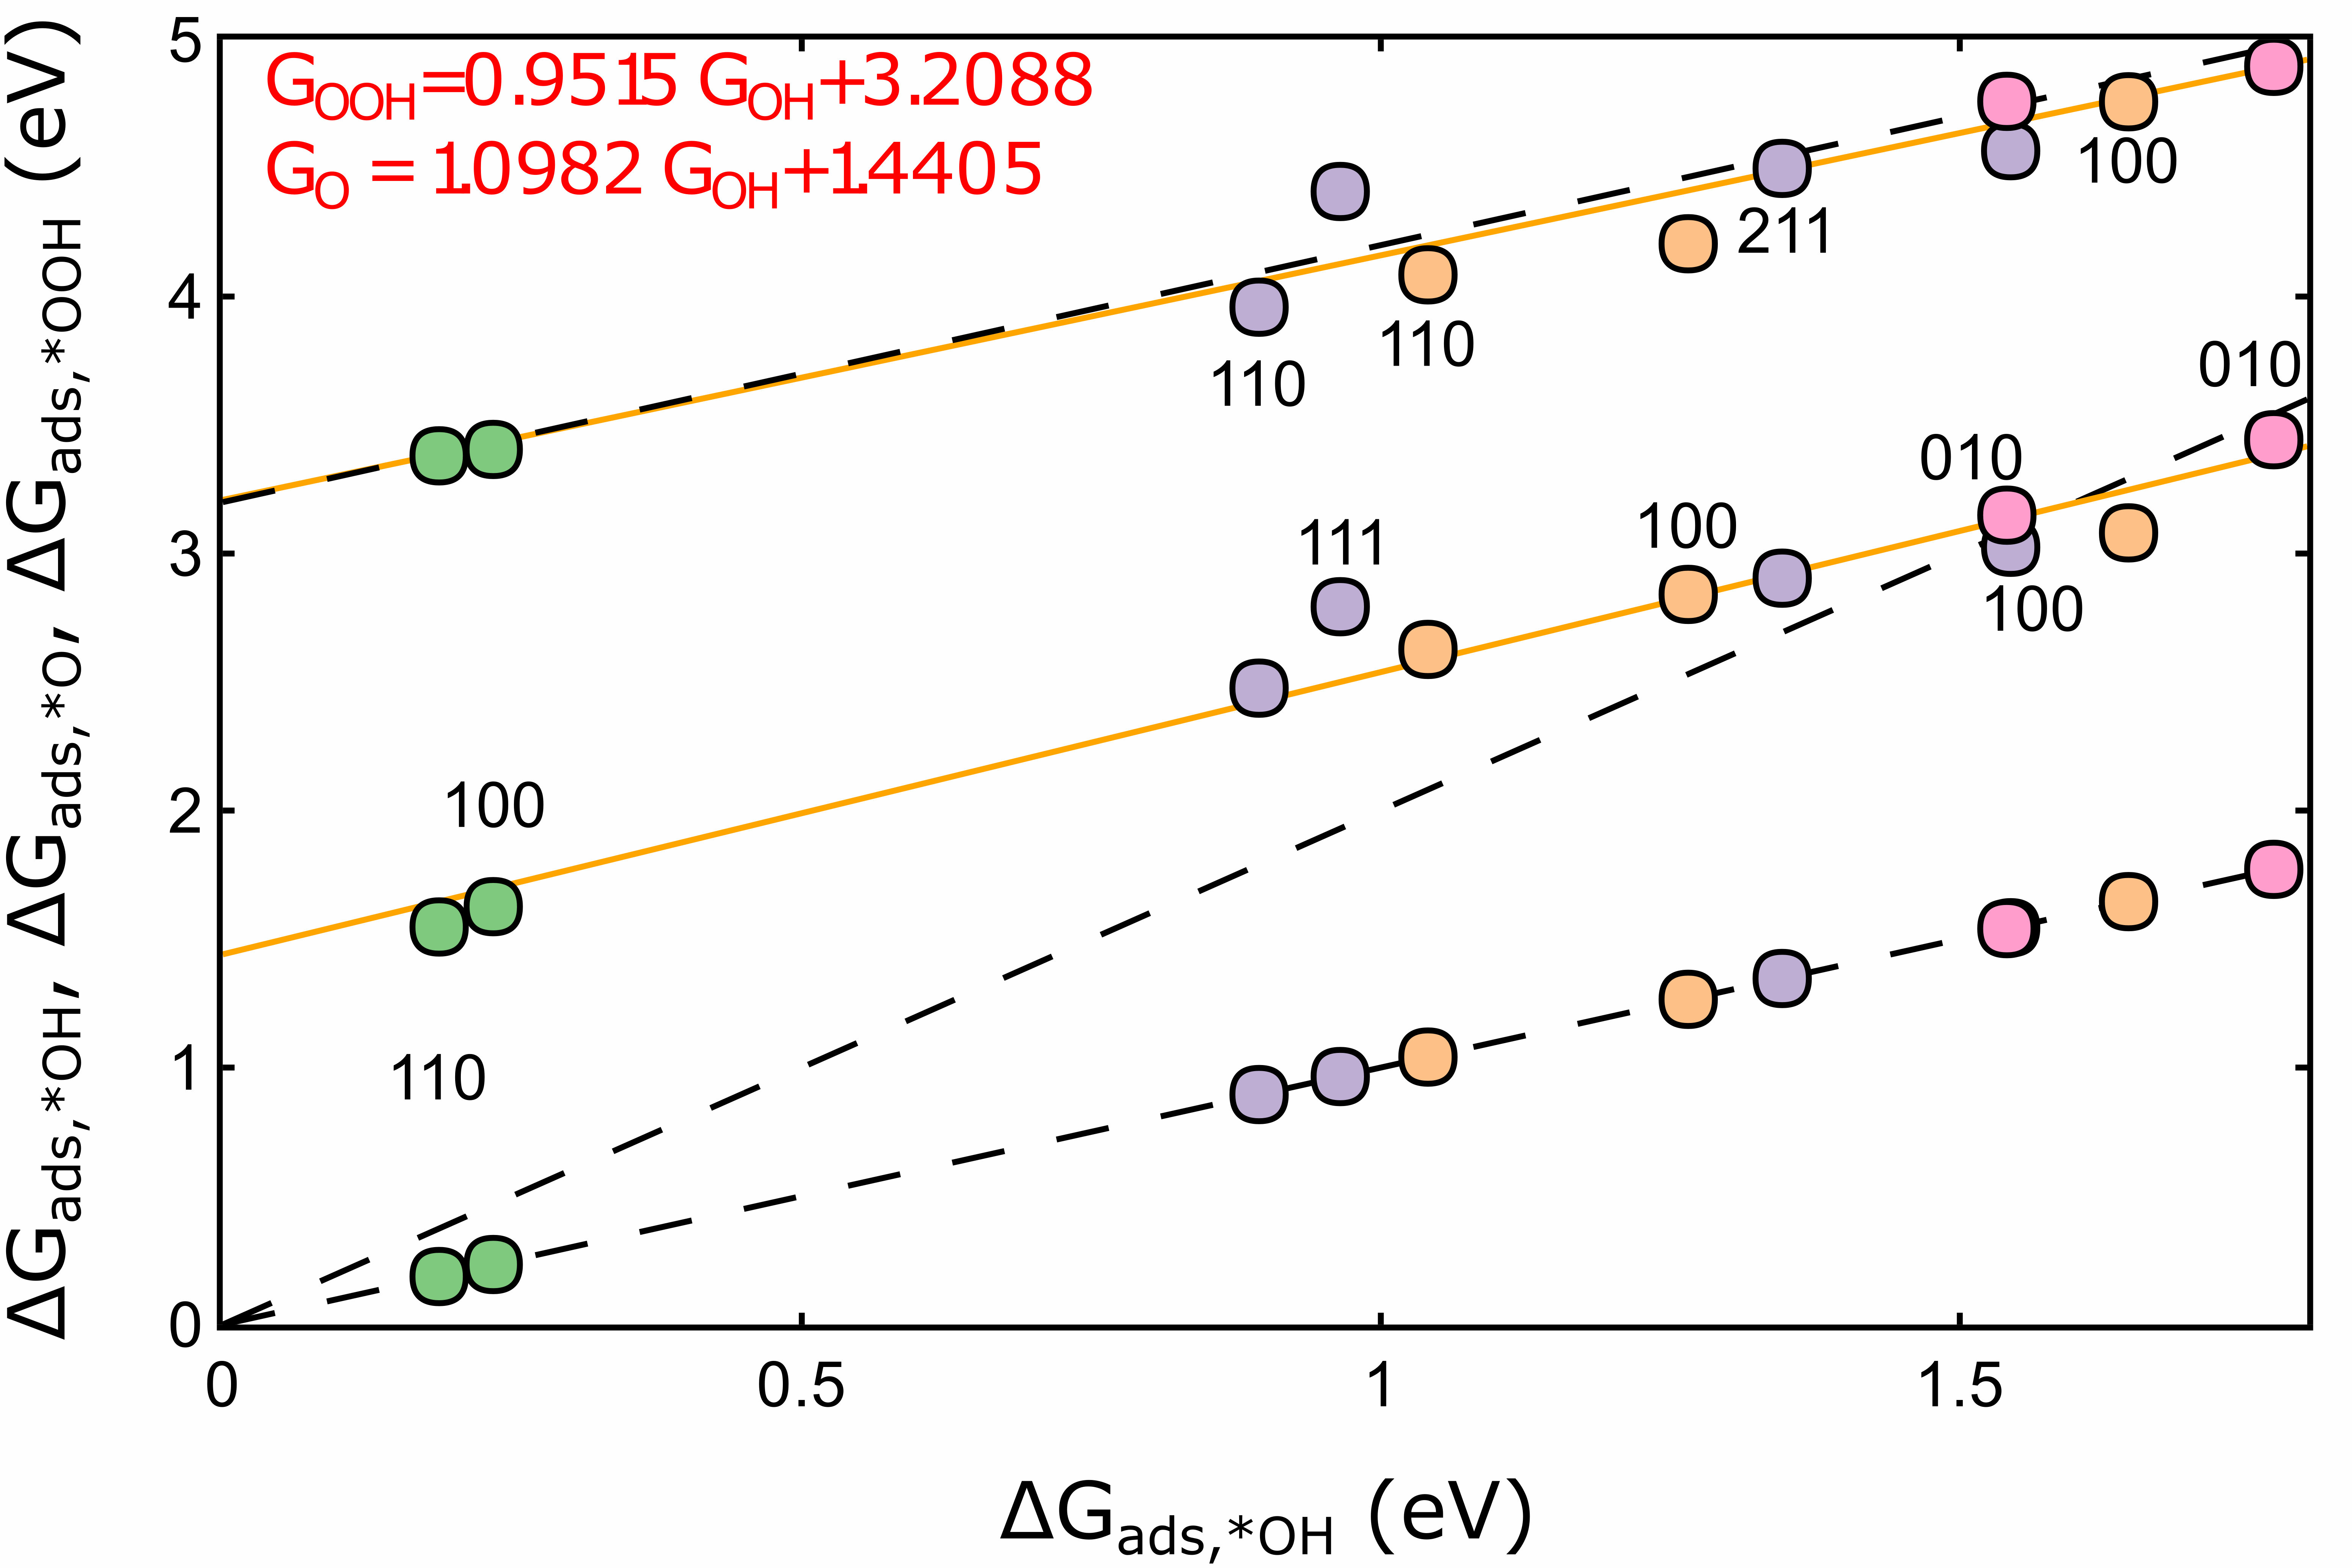
\includegraphics
{02_figures/oer_activity_stability/00_master__oer_scaling__main_v0__outplot2.png}
}
\caption{\label{fig:scaling_relations}
% Adsorption free energy scaling relations plot.
Relationship between the adsorption free energies of the three key OER intermediates (*OH, *O, *OOH), with \DGOH chosen as the dependent variable.
Best fit lines are provided for \DGOOH vs. \DGOH and \DGO vs. \DGOH.
%
Additionally, ``universal scaling relations'' for \DGOOH vs. \DGOH and \DGO vs. \DGOH are shown (black dotted lines) to emphasize our deviation from the traditionally reported scaling fits.
The \DGOH line is  shown as guide to eye.
% TODO Do I have to redefine the color convention every caption?
}
\end{figure*}
% __|

% ################################# Paragraph #################################
% %%%%%%%%%%%%%%%%%%%%%%%%%%%%%%%%%%%%%%%%%%%%%%%%%%%%%%%%%%%%%%%%%%%%%%%%%%%%%
%
% %%%%%%%%%%%%%%%%%%%%%%%%%%%%%%%%%%%%%%%%%%%%%%%%%%%%%%%%%%%%%%%%%%%%%%%%%%%%%


% __|



% %%%%%%%%%%%%%%%%%%%%%%%%%%%%%%%%%%%%%%%%%%%%%%%%%%%%%%%%%%%%%%%%%%%%%%%%%%%%%
\subsection{Bulk Systems}  % %%%%%%%%%%%%%%%%%%%%%%%%%%%%%%%%%%%%%%%%%%%%%%%%%%
% %%%%%%%%%%%%%%%%%%%%%%%%%%%%%%%%%%%%%%%%%%%%%%%%%%%%%%%%%%%%%%%%%%%%%%%%%%%%%
%
% %%%%%%%%%%%%%%%%%%%%%%%%%%%%%%%%%%%%%%%%%%%%%%%%%%%%%%%%%%%%%%%%%%%%%%%%%%%%%
% %%%%%%%%%%%%%%%%%%%%%%%%%%%%%%%%%%%%%%%%%%%%%%%%%%%%%%%%%%%%%%%%%%%%%%%%%%%%%
% | - Bulk Systems
% Formation energies of 4 polymorphs

% __|



% %%%%%%%%%%%%%%%%%%%%%%%%%%%%%%%%%%%%%%%%%%%%%%%%%%%%%%%%%%%%%%%%%%%%%%%%%%%%%
\subsection{Table of OER energetics}  % %%%%%%%%%%%%%%%%%%%%%%%%%%%%%%%%%%%%%%%
% %%%%%%%%%%%%%%%%%%%%%%%%%%%%%%%%%%%%%%%%%%%%%%%%%%%%%%%%%%%%%%%%%%%%%%%%%%%%%
%
% %%%%%%%%%%%%%%%%%%%%%%%%%%%%%%%%%%%%%%%%%%%%%%%%%%%%%%%%%%%%%%%%%%%%%%%%%%%%%
% %%%%%%%%%%%%%%%%%%%%%%%%%%%%%%%%%%%%%%%%%%%%%%%%%%%%%%%%%%%%%%%%%%%%%%%%%%%%%
% | - Table of OER energetics

% __|

% __|
